\begin{figure}[t]
    \centering
    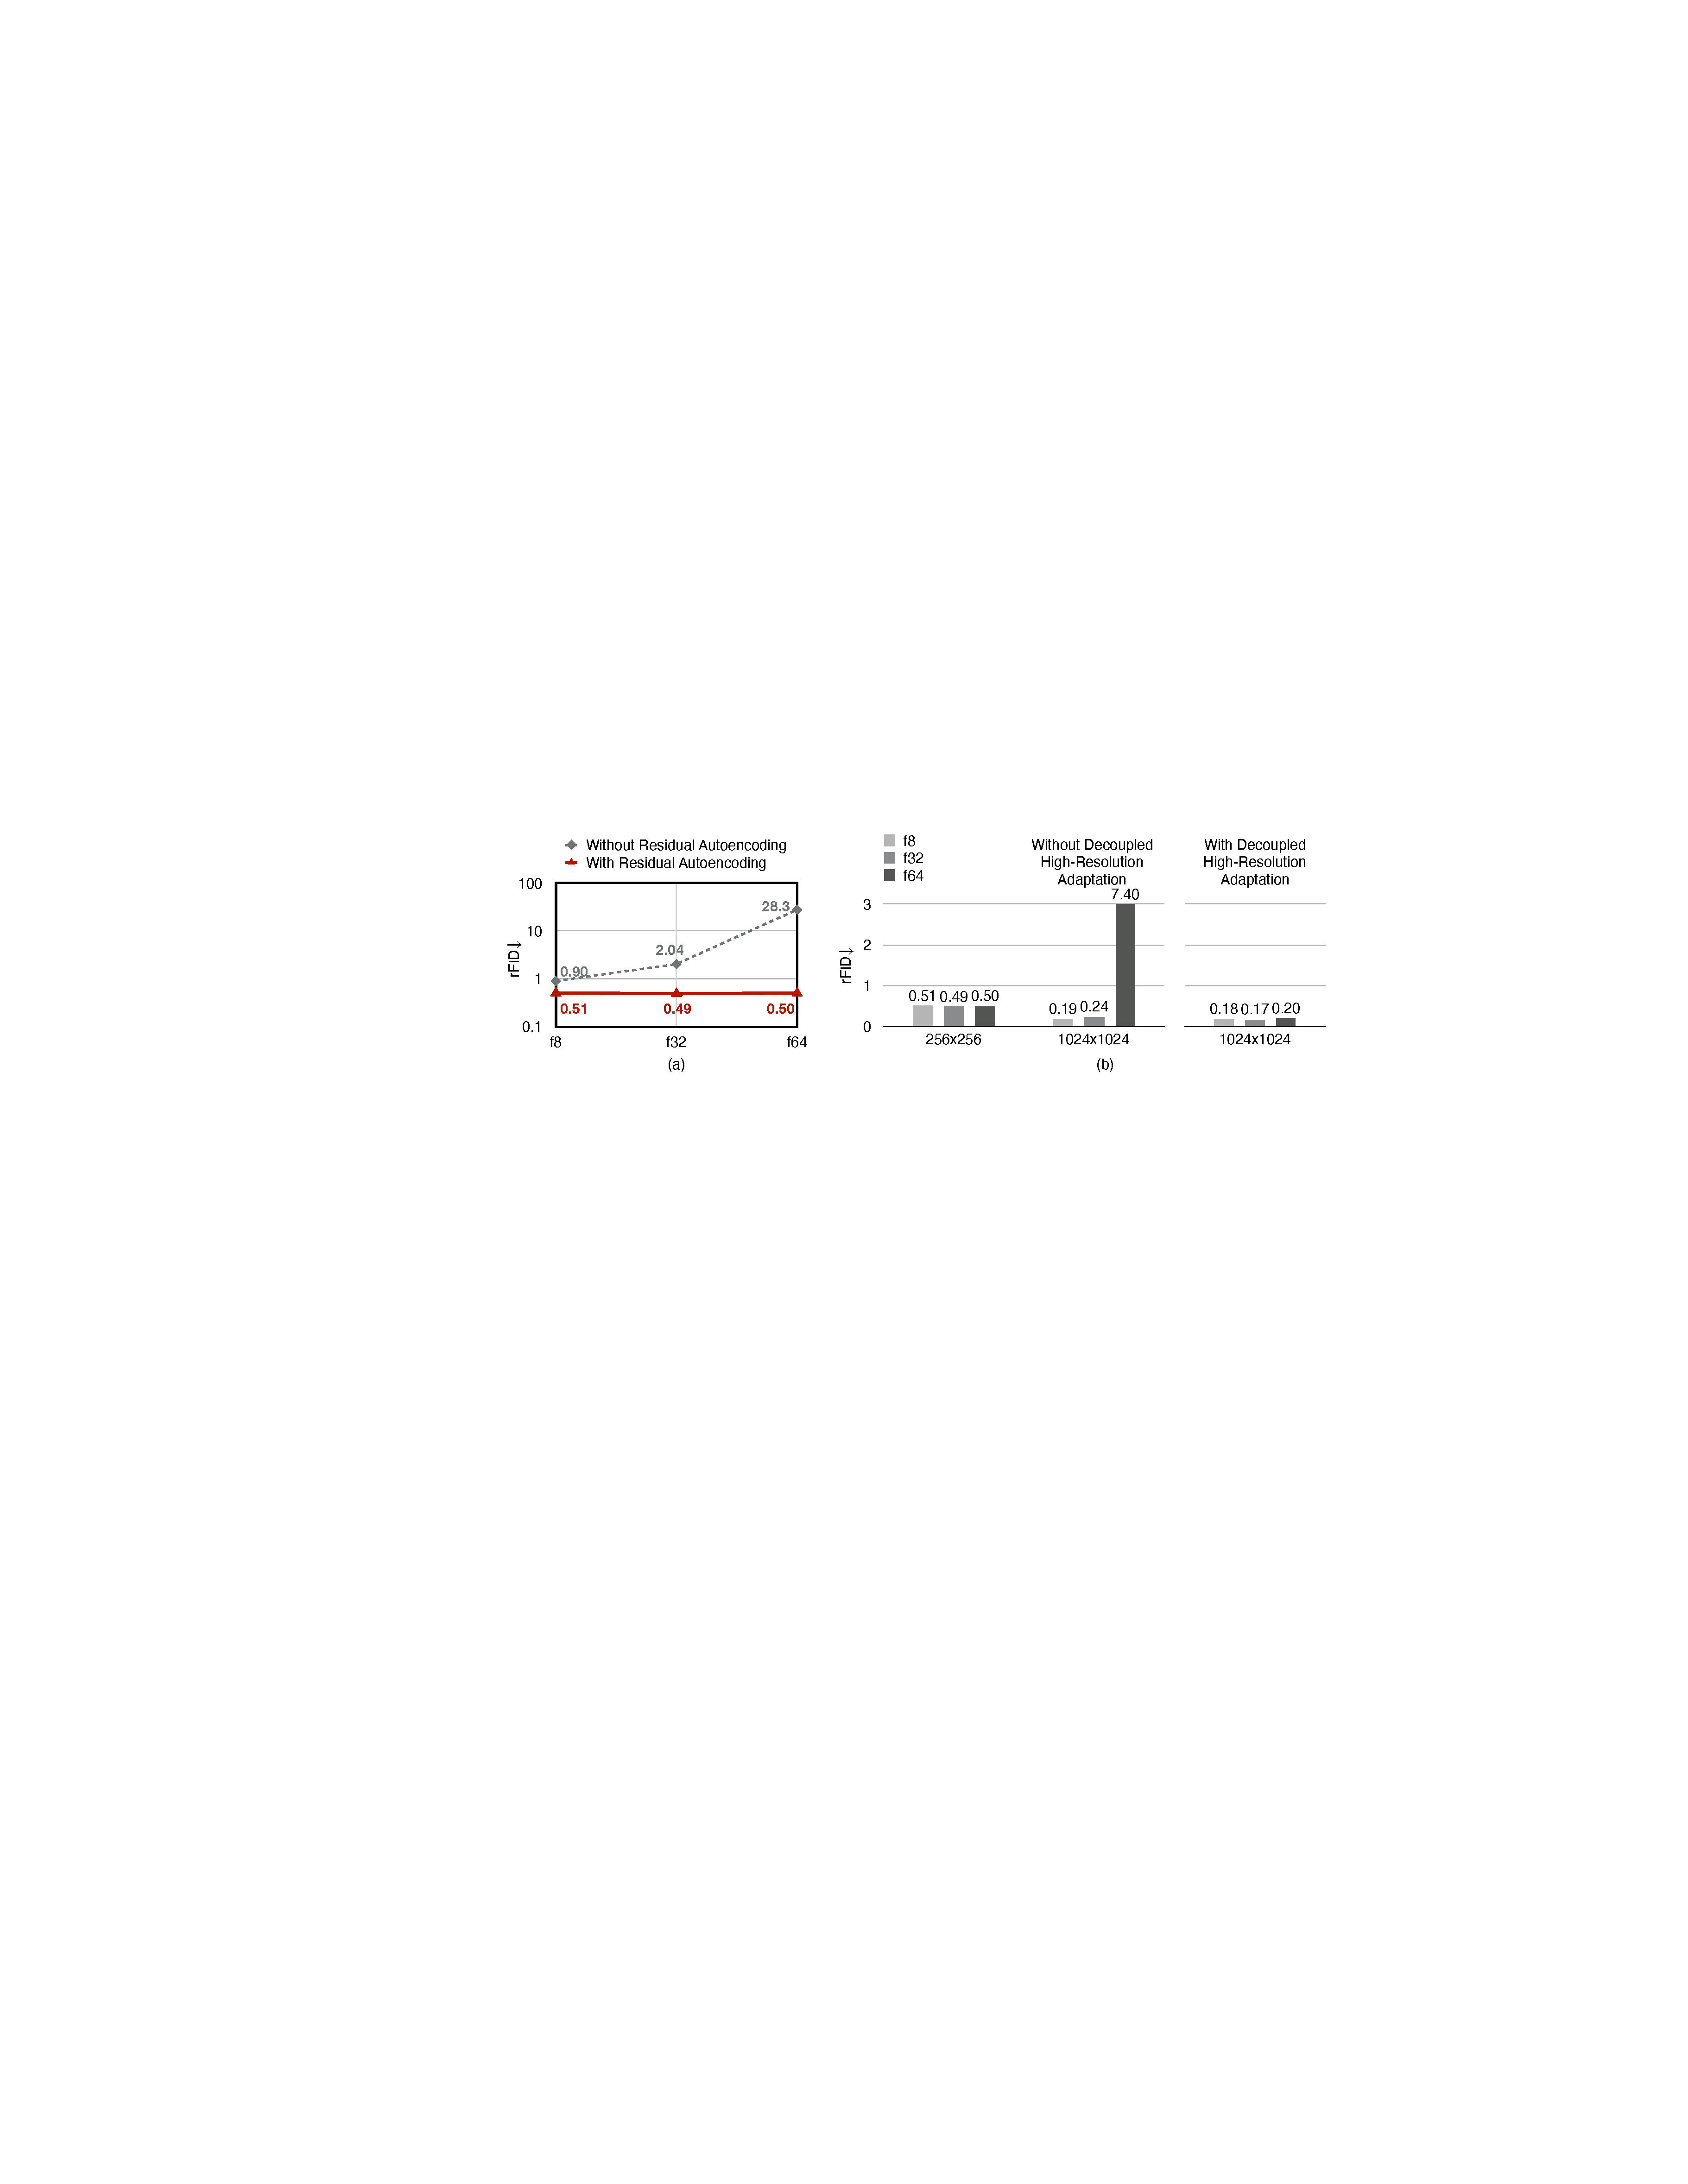
\includegraphics[width=1\linewidth]{figures/src/method_motivation.pdf}
    \vspace{-15pt}
    \caption{(a) High spatial-compression autoencoders are more difficult to optimize. Even with the same latent shape and stronger learning capacity, it still cannot match the f8 autoencoder's rFID. (b) High spatial-compression autoencoders suffer from significant reconstruction accuracy drops when generalizing from low-resolution to high-resolution. }
    \vspace{-10pt}
    \label{fig:method_motivation}
\end{figure}

\section{Method}
\label{sec:method}
\vspace{-5pt}
In this section, we first analyze why existing high spatial-compression autoencoders (e.g., SD-VAE-f64) fail to match the accuracy of low spatial-compression autoencoders (e.g., SD-VAE-f8). Then we introduce our \modelfull (\modelshort) with \emph{Residual Autoencoding} and \emph{Decoupled High-Resolution Adaptation} to close the accuracy gap. Finally, we discuss the applications of our \modelshort to latent diffusion models. 

\subsection{Motivation}\label{sec:motivation}
We conduct ablation study experiments to get insights into the underlying source of the accuracy gap between high spatial-compression and low spatial-compression autoencoders. Specifically, we consider three settings with gradually increased spatial compression ratio, from f8 to f64. 

Each time the spatial compression ratio increases, we stack additional encoder and decoder stages upon the current autoencoder. In this way, high spatial-compression autoencoders contain low spatial-compression autoencoders as sub-networks and thus have higher learning capacity.

Additionally, we increase the latent channel number to maintain the same total latent size across different settings. We can then convert the latent to a higher spatial compression ratio one by applying a space-to-channel operation \citep{shi2016real}: $H \times W \times C \rightarrow \frac{H}{p} \times \frac{W}{p} \times p^2C$. 

We summarize the results in Figure~\ref{fig:method_motivation} (a, gray dash line). Even with the same total latent size and stronger learning capacity, we still observe degraded reconstruction accuracy when the spatial compression ratio increases. It demonstrates that \emph{the added encoder and decoder stages (consisting of multiple SD-VAE building blocks) work worse than a simple space-to-channel operation}. 

Based on this finding, we conjecture \emph{the accuracy gap comes from the model learning process: while we have good local optimums in the parameter space, the optimization difficulty hinders high spatial-compression autoencoders from reaching such local optimums.}

\begin{figure}[t]
    \centering
    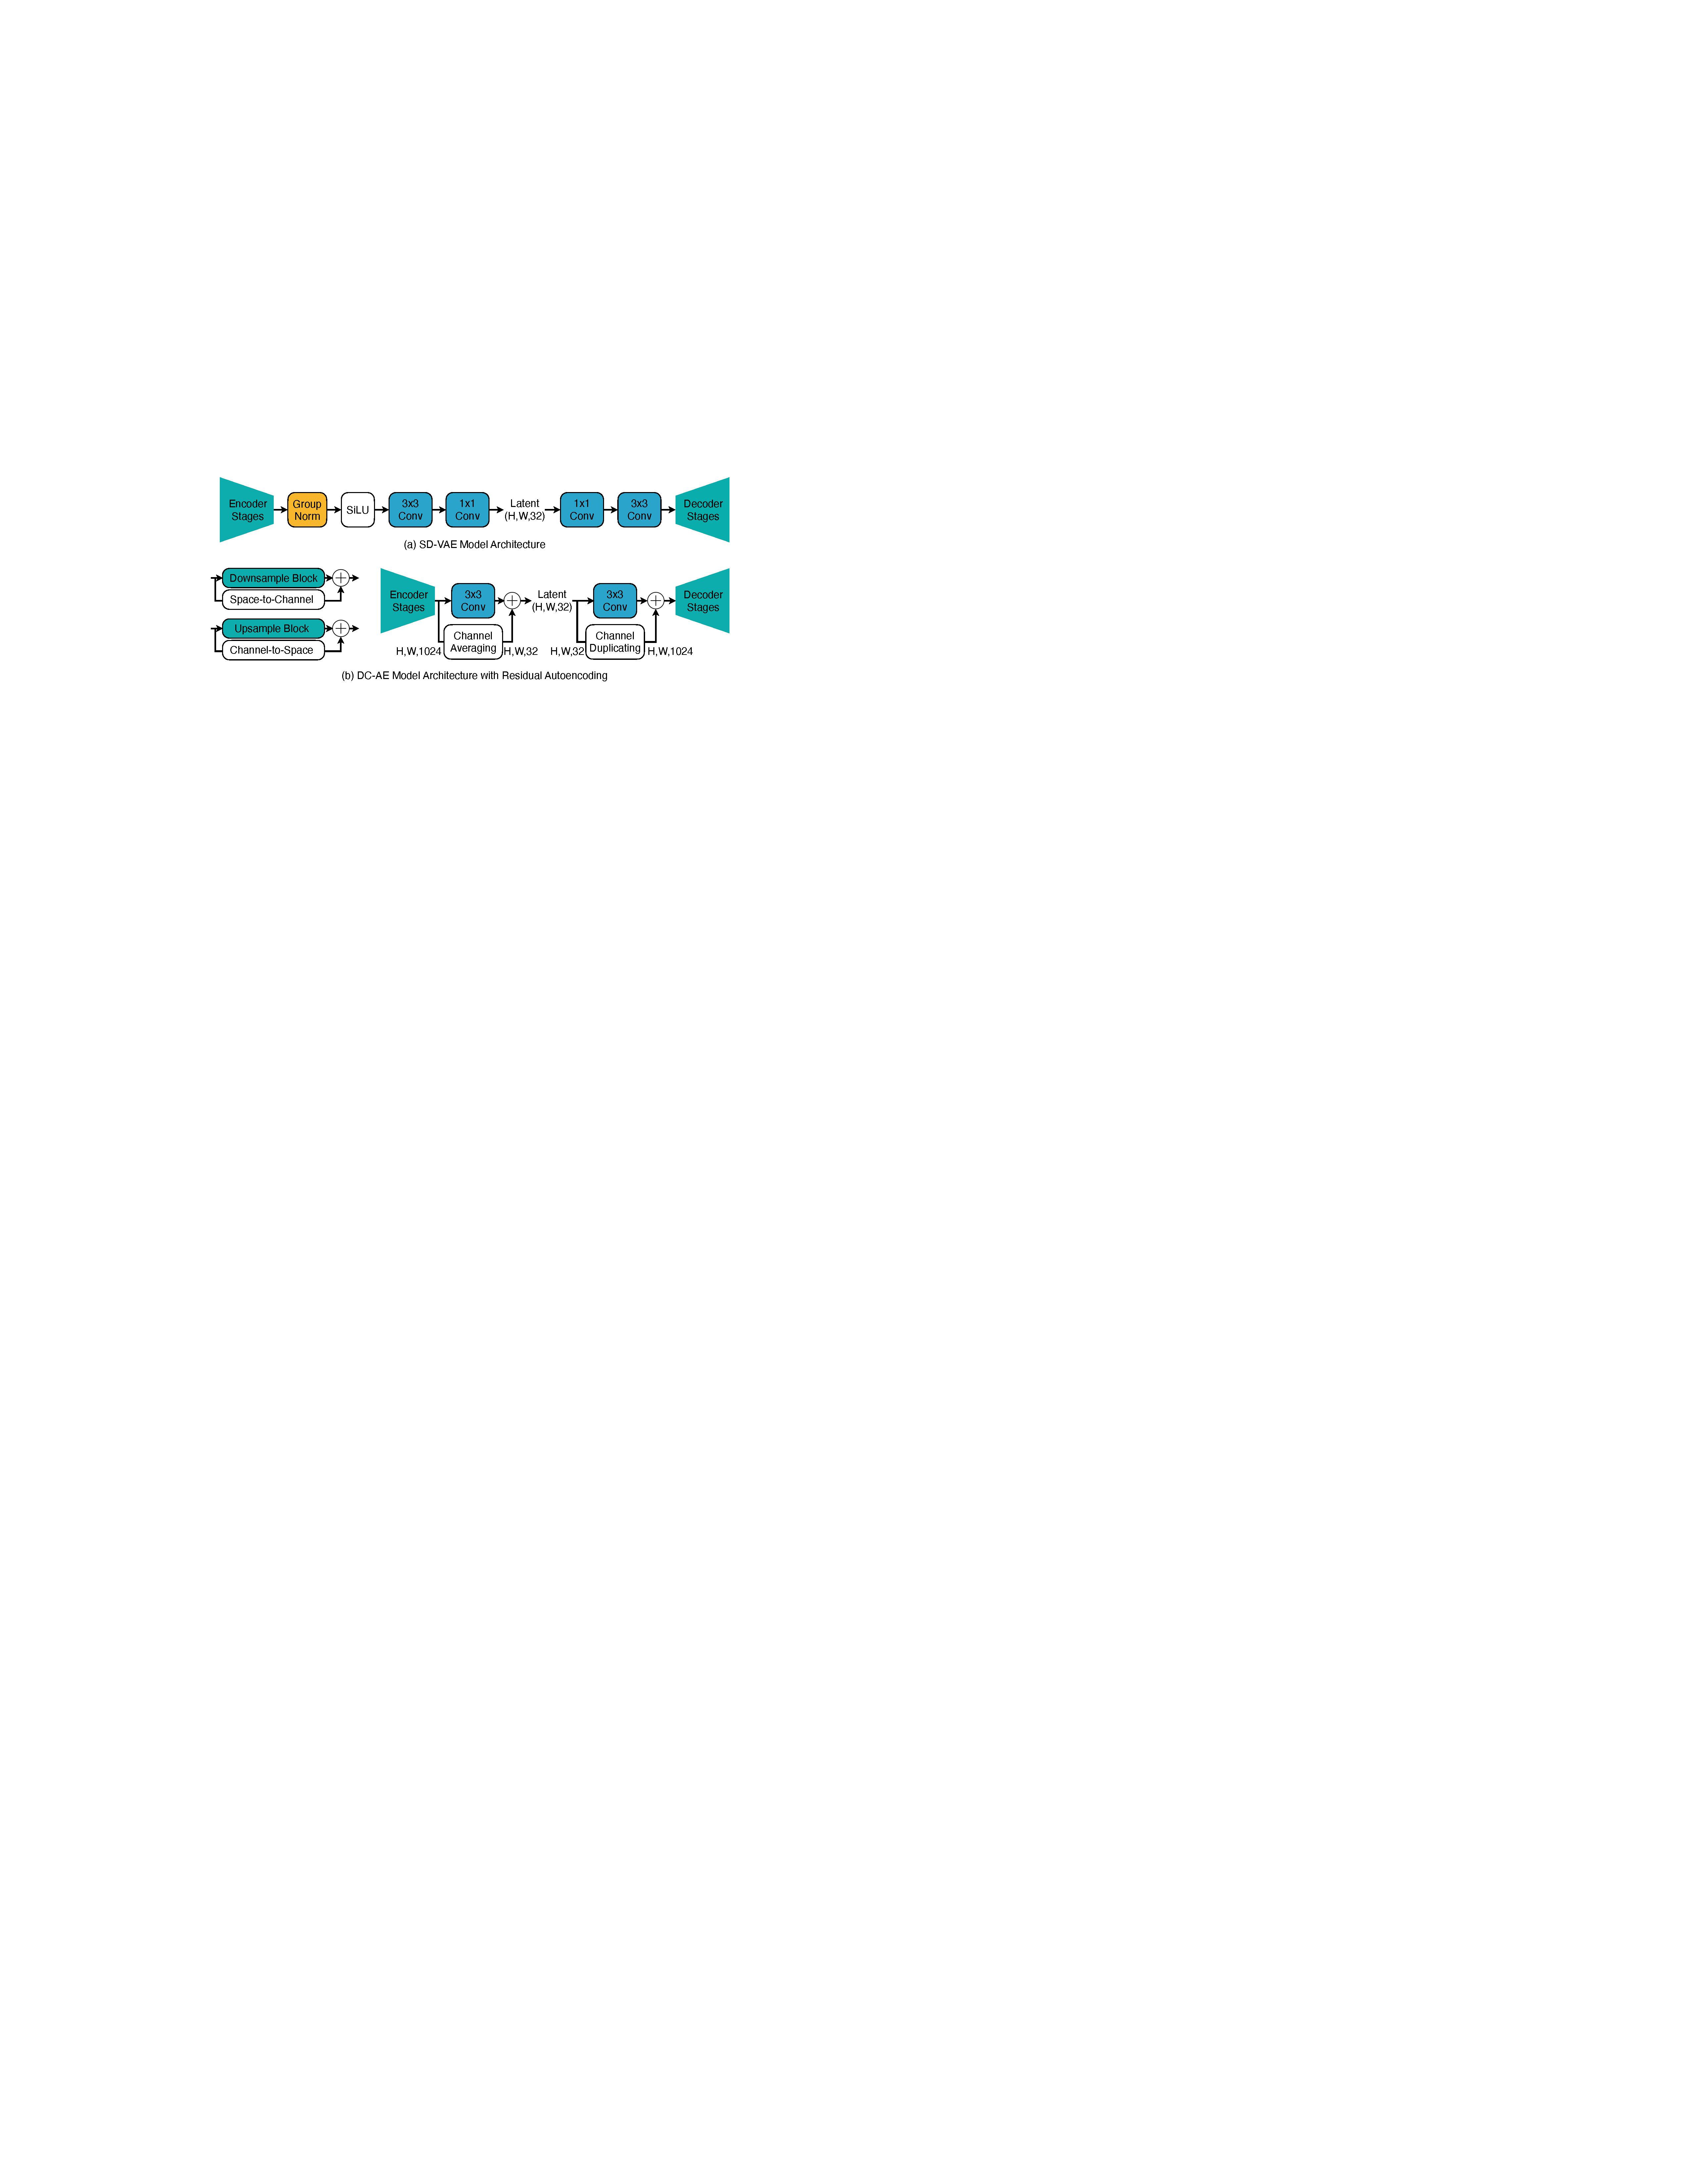
\includegraphics[width=0.9\linewidth]{figures/src/method_arch.pdf}
    \caption{\textbf{Illustration of Residual Autoencoding.} It adds non-parametric shortcuts to let the neural network modules learn residuals based on the space-to-channel operation.}
    \label{fig:method_arch}
\end{figure}

\subsection{\modelfull}\label{sec:main_model}
\paragraph{Residual Autoencoding.} Motivated by the analysis, we introduce Residual Autoencoding to address the accuracy gap. The general idea is depicted in Figure~\ref{fig:method_arch}. The core difference from the conventional design is that we explicitly let neural network modules learn the downsample residuals based on the space-to-channel operation to alleviate the optimization difficulty. Different from ResNet \citep{he2016deep}, the residual here is not identity mapping, but space-to-channel mapping.

In practice, this is implemented by adding extra non-parametric shortcuts on the encoder's downsample blocks and decoder's upsample blocks (Figure~\ref{fig:method_arch} b, left). Specifically, for the downsample block, the non-parametric shortcut is a space-to-channel operation followed by a non-parametric channel averaging operation to match the channel number. For example, assuming the downsample block's input feature map shape is $H \times W \times C$ and its output feature map shape is $\frac{H}{2} \times \frac{W}{2} \times 2C$, then the added shortcut is:

{\small
\begin{align}
    H \times W \times C & \xrightarrow{\text{space-to-channel}} \frac{H}{2} \times \frac{W}{2} \times 4C \nonumber \\
    & \underbrace{\xrightarrow{\text{split into two groups}} [\frac{H}{2} \times \frac{W}{2} \times 2C, \frac{H}{2} \times \frac{W}{2} \times 2C] \xrightarrow{\text{average}} \frac{H}{2} \times \frac{W}{2} \times 2C.}_{\text{channel averaging}} \nonumber
\end{align}
}

Accordingly, for the upsample block, the non-parametric shortcut is a channel-to-space operation followed by a non-parametric channel duplicating operation:

{\small
\begin{align}
    \frac{H}{2} \times \frac{W}{2} \times 2C & \xrightarrow{\text{channel-to-space}}  \nonumber H \times W \times \frac{C}{2} \\
    & \underbrace{\xrightarrow{\text{duplicate}} [H \times W \times \frac{C}{2}, H \times W \times \frac{C}{2}] \xrightarrow{\text{concat}} H \times W \times C.}_{\text{channel duplicating}} \nonumber
\end{align}
}

In addition to the downsample and upsample blocks, we also change the middle stage design following the same principle (Figure~\ref{fig:method_arch} b, right). 

Figure~\ref{fig:method_motivation} (a) shows the comparison with and without our Residual Autoencoding on ImageNet $256 \times 256$. We can see that Residual Autoencoding effectively improves the reconstruction accuracy of high spatial-compression autoencoders. 

\begin{figure}[t]
    \centering
    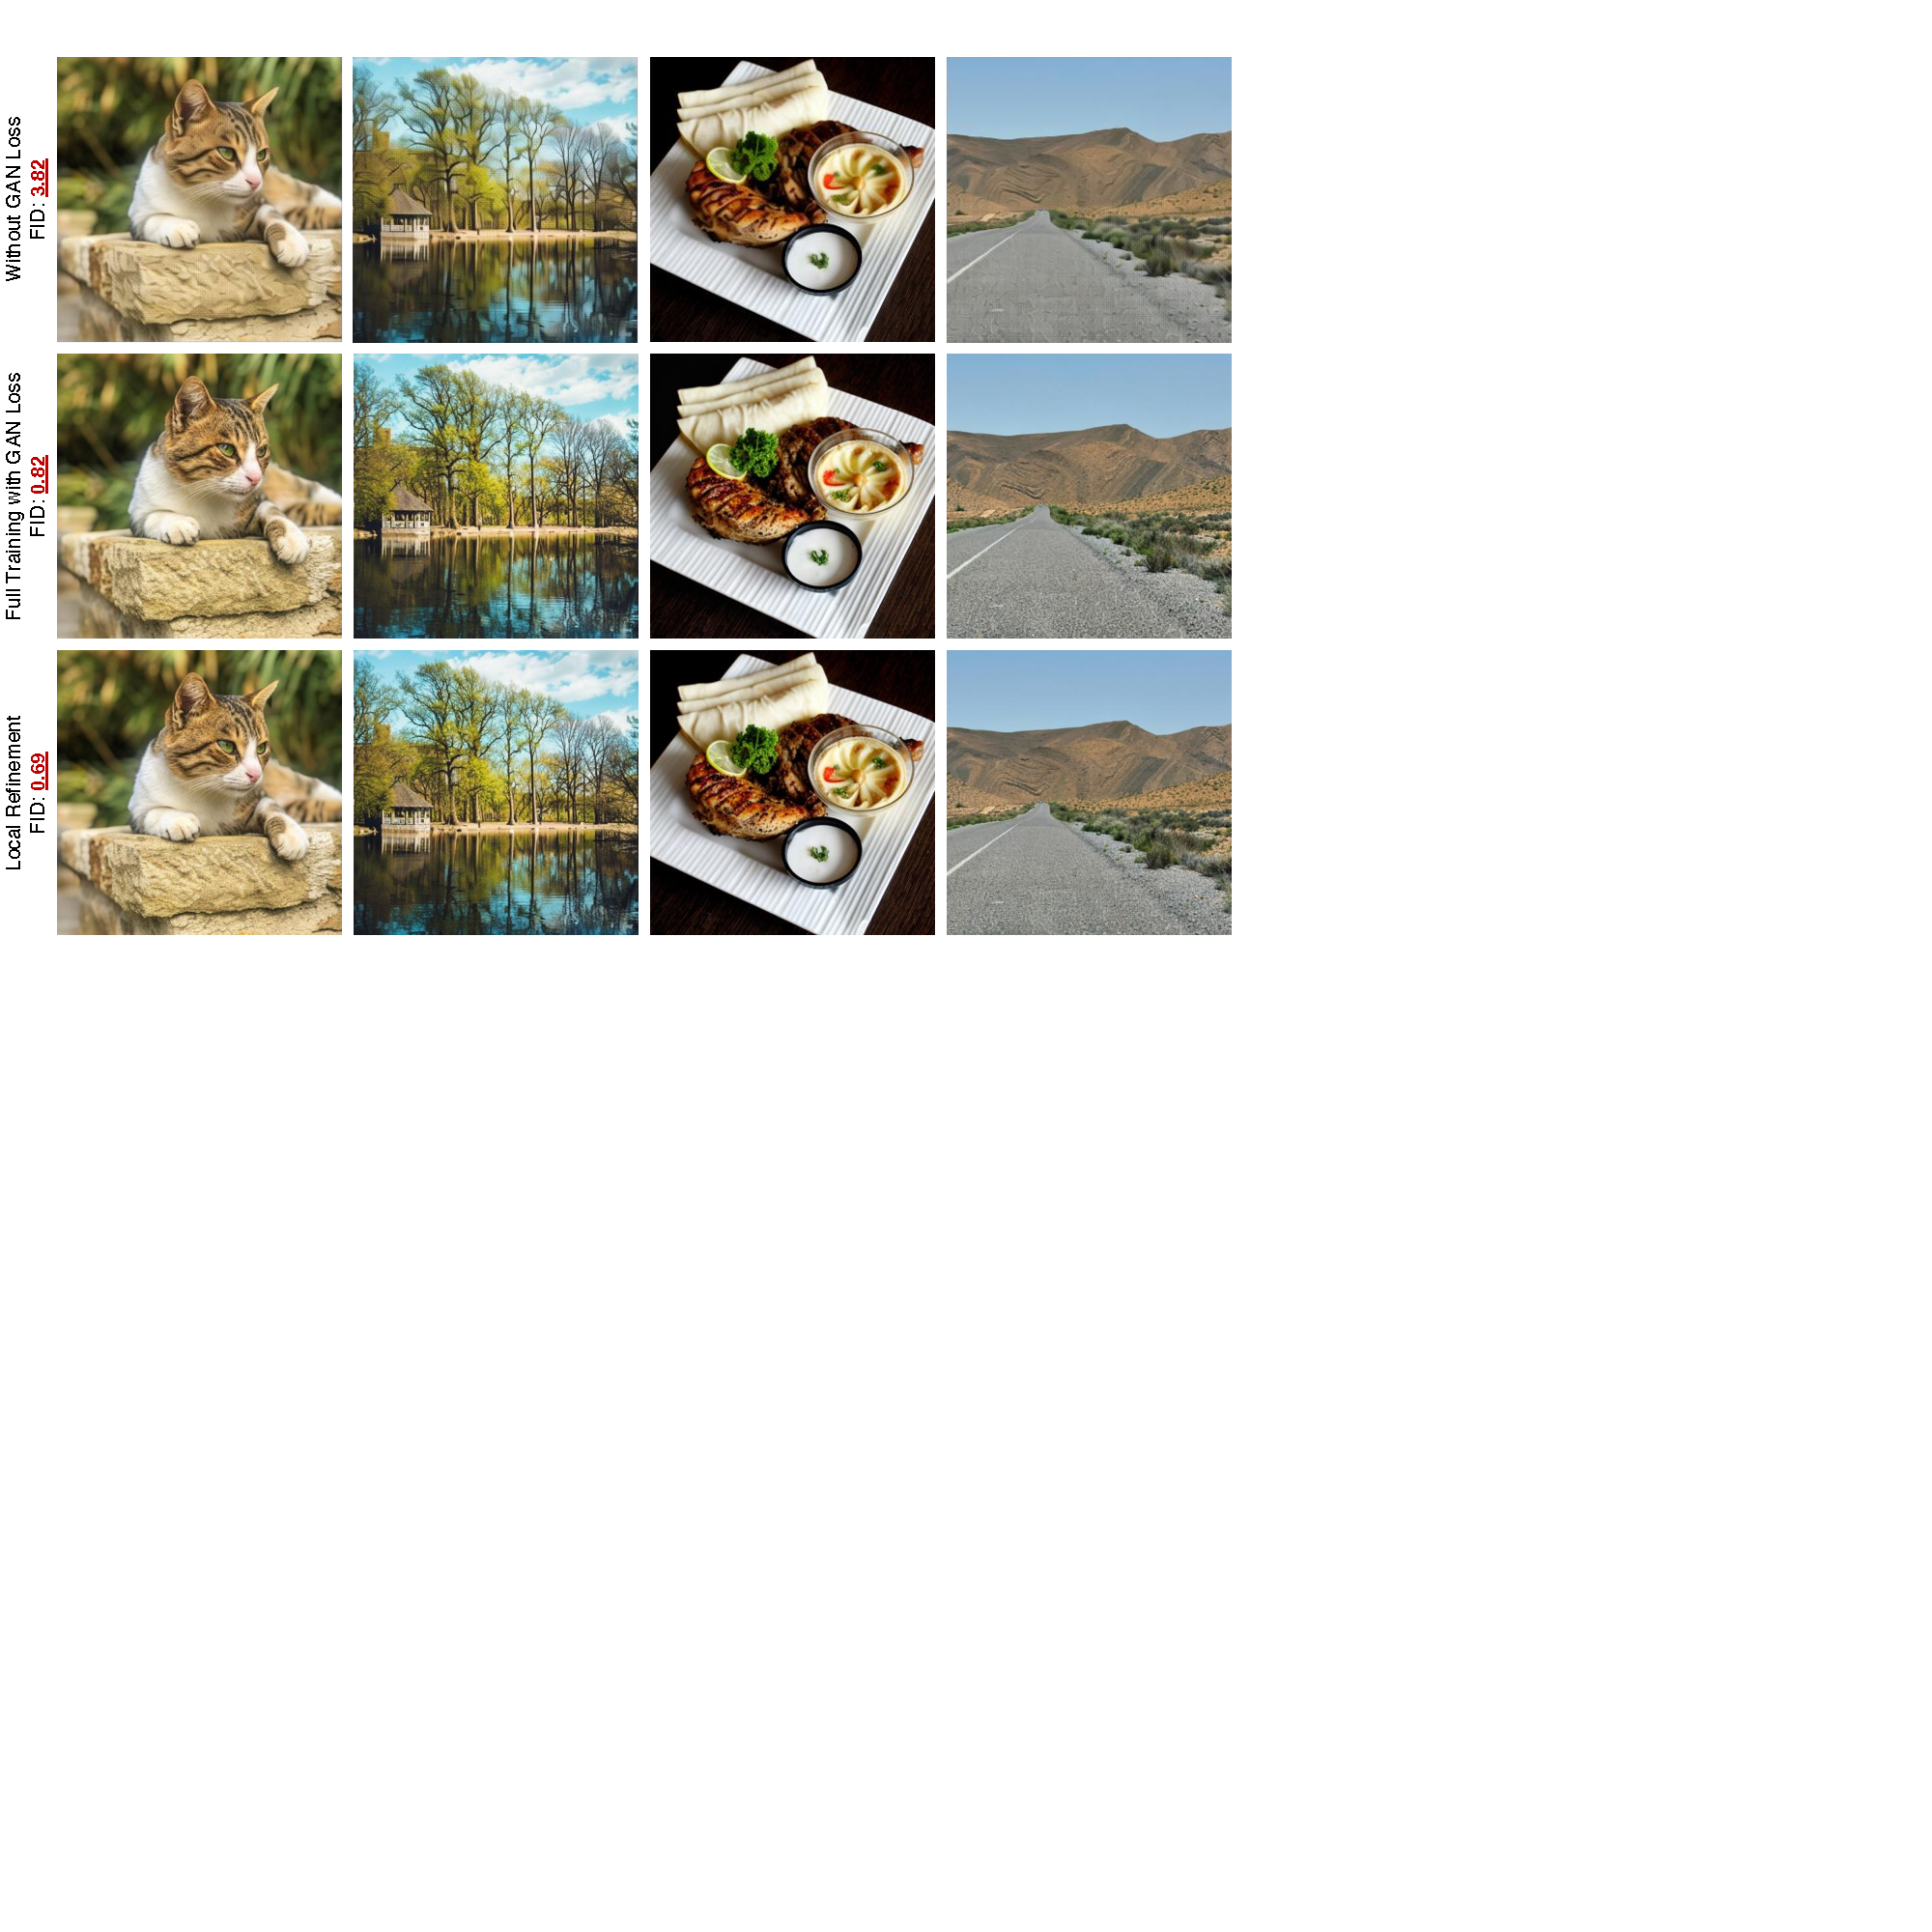
\includegraphics[width=0.95\linewidth]{figures/src/method_gan.pdf}
    \caption{Autoencoder already learns to reconstruct content and semantics without GAN loss, while GAN loss improves local details and removes local artifacts. We replace the GAN loss full training with lightweight local refinement training which achieves the same goal and has lower training cost.}
    \label{fig:method_gan}
\end{figure}
\begin{figure}[t]
    \centering
    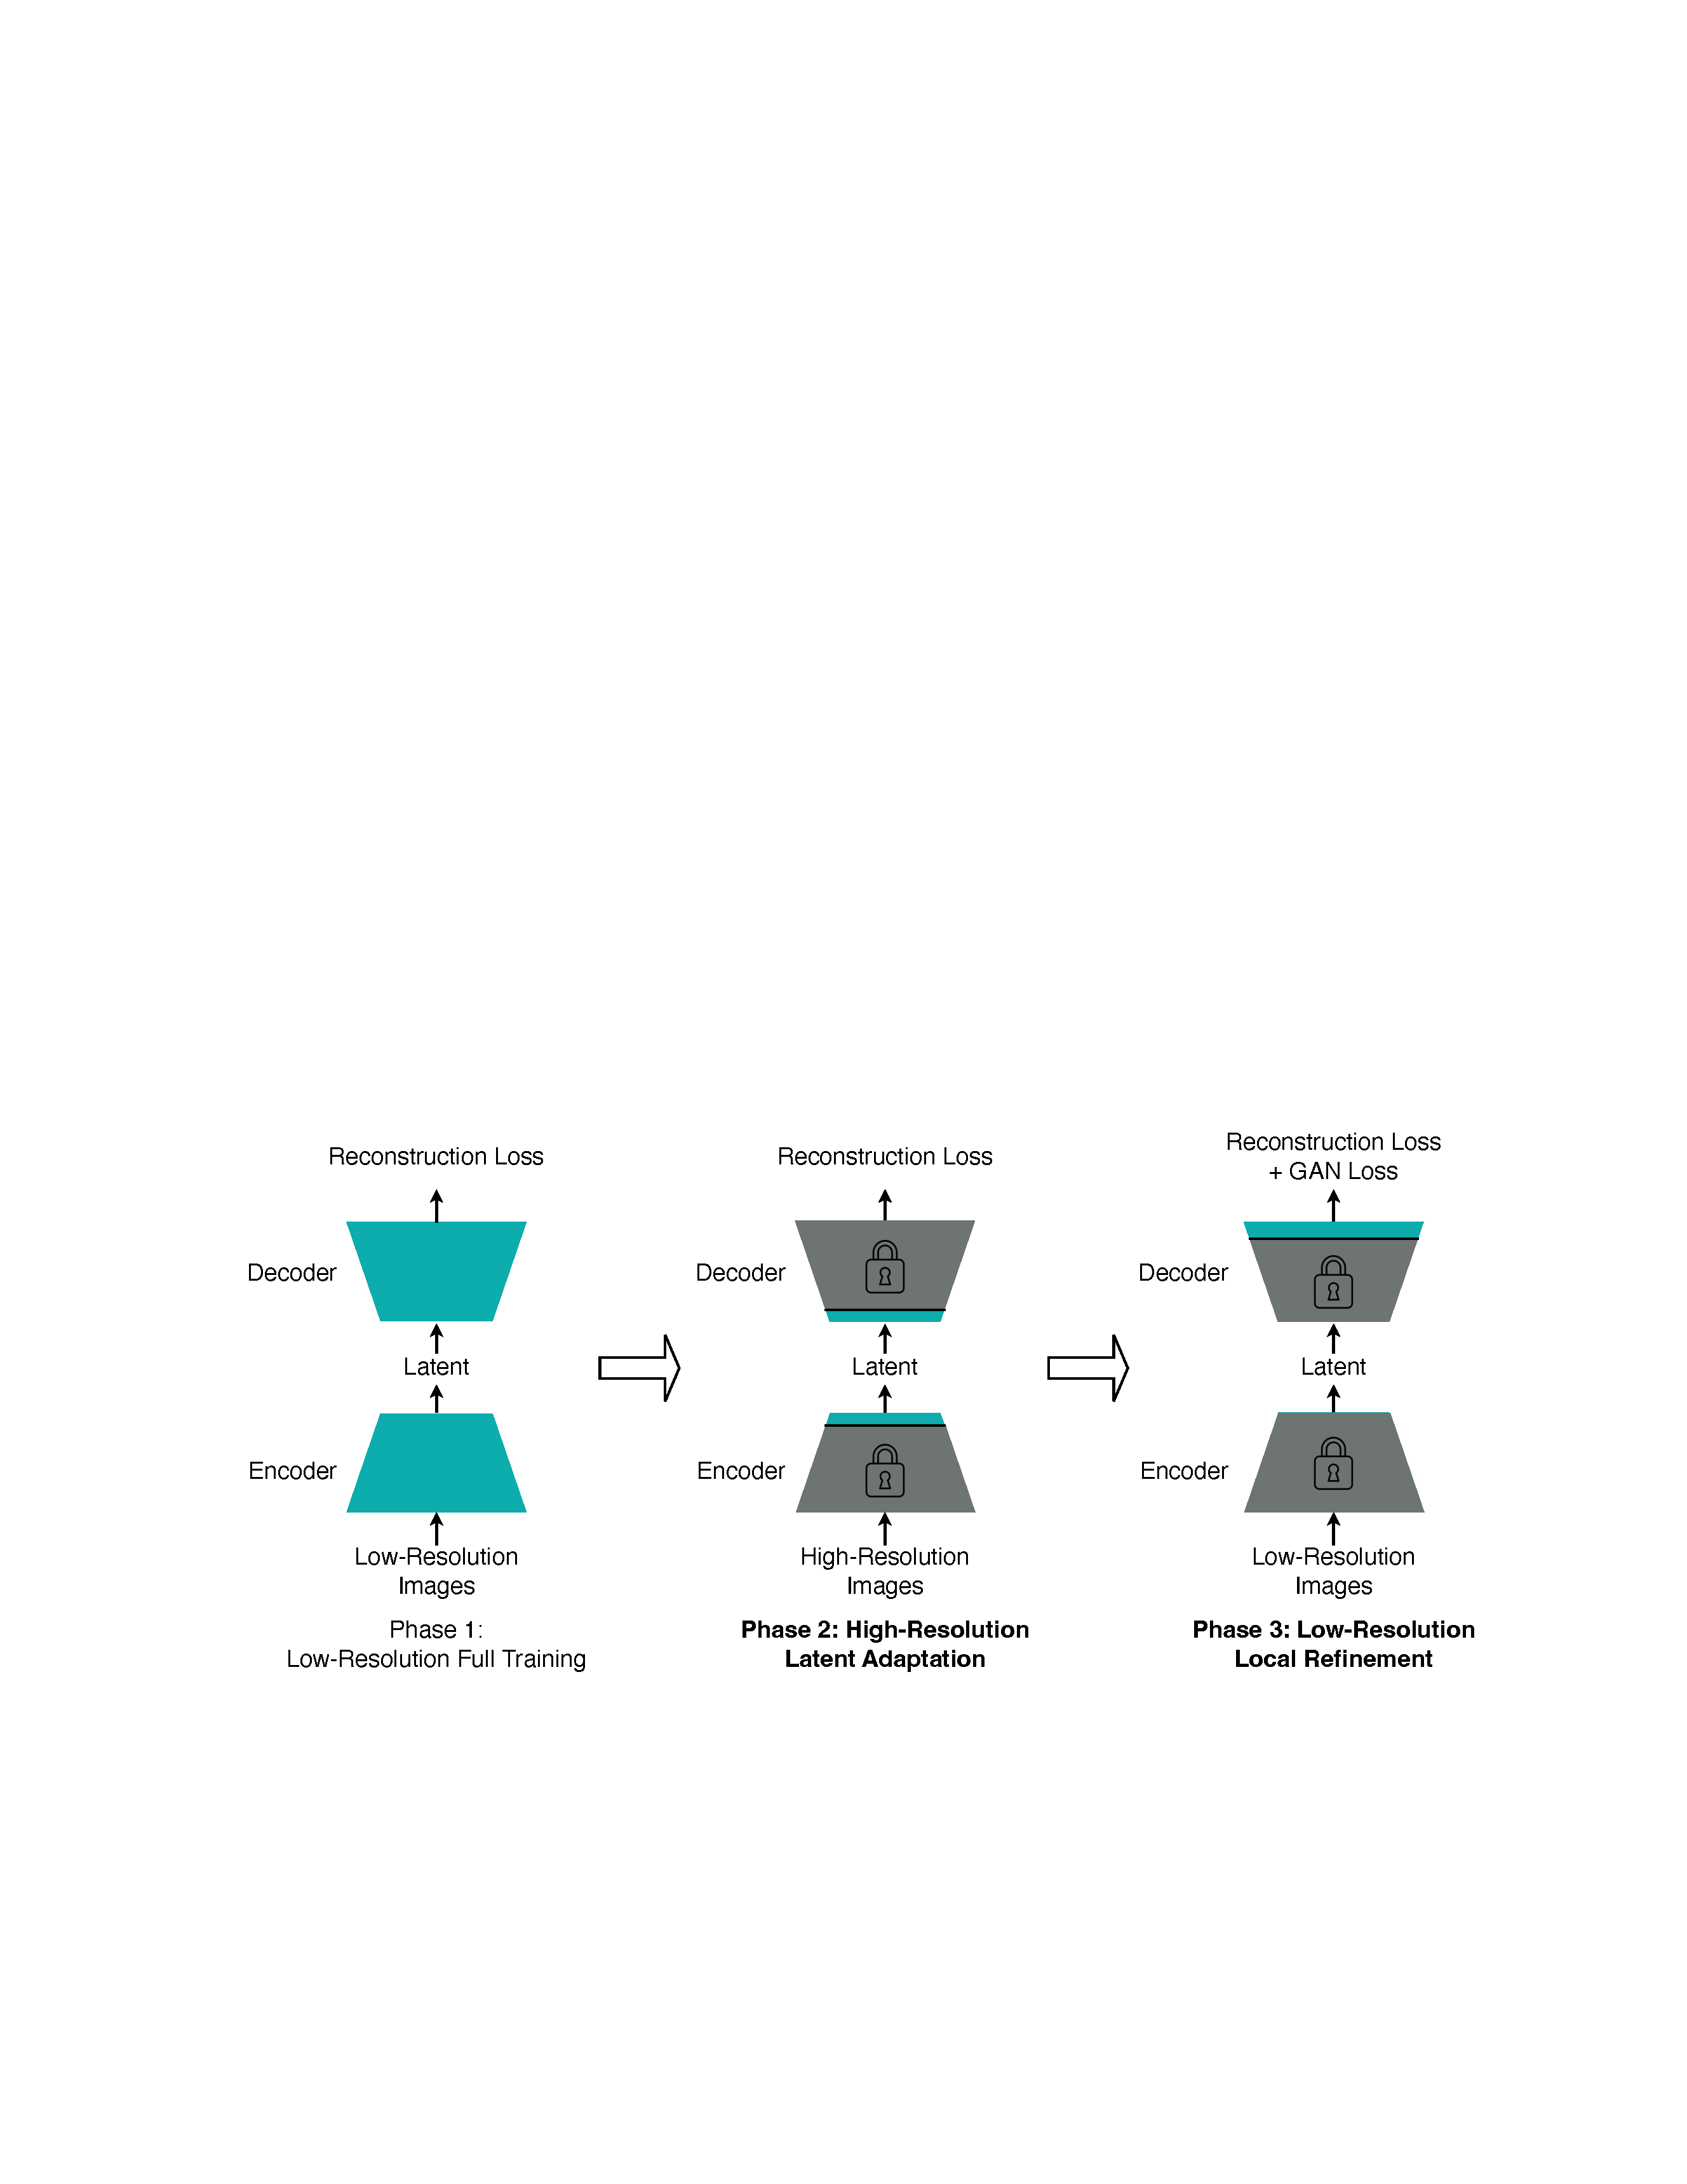
\includegraphics[width=0.95\linewidth]{figures/src/method_training_pipeline.pdf}
    \caption{\textbf{Illustration of Decoupled High-Resolution Adaptation.}}
    \label{fig:method_training_pipeline}
\end{figure}

\paragraph{Decoupled High-Resolution Adaptation.} Residual Autoencoding alone can address the accuracy gap when handling low-resolution images. However, when extending it to high-resolution images, we find it not sufficient. Due to the large cost of high-resolution training, the common practice for high-resolution diffusion models is directly using autoencoders trained on low-resolution images (e.g., $256\times256$) \citep{chenpixart,chen2024pixart}. This strategy works well for low spatial-compression autoencoders. However, high spatial-compression autoencoders suffer from a significant accuracy drop. For example, in Figure~\ref{fig:method_motivation} (b), we can see that f64 autoencoder's rFID degrades from 0.50 to 7.40 when generalizing from $256\times256$ to $1024\times1024$. In contrast, the f8 autoencoder's rFID improves from 0.51 to 0.19 under the same setting. Additionally, we also find this issue more severe when using a higher spatial compression ratio. In this work, we refer to this phenomenon as the \emph{generalization penalty of high spatial-compression autoencoders}. A straightforward solution to address this issue is conducting training on high-resolution images. However, it suffers from a large training cost and unstable high-resolution GAN loss training. 

We introduce Decoupled High-Resolution Adaptation to tackle this challenge. Figure~\ref{fig:method_training_pipeline} demonstrates the detailed training pipeline. Compared with the conventional single-phase training strategy \citep{rombach2022high}, our Decoupled High-Resolution Adaptation has two key differences. 

First, we decouple the GAN loss training from the full model training and introduce a dedicated local refinement phase for the GAN loss training. In the local refinement phase (Figure~\ref{fig:method_training_pipeline}, phase 3), we only tune the head layers of the decoder while freezing all the other layers. The intuition of this design is based on the finding that the reconstruction loss alone is sufficient for learning to reconstruct the content and semantics. Meanwhile, the GAN loss mainly improves local details and removes local artifacts (Figure~\ref{fig:method_gan}). Achieving the same goal of local refinement, only tuning the decoder's head layers has a lower training cost and delivers better accuracy than the full training. 

Moreover, the decoupling prevents the GAN loss training from changing the latent space. This approach enables us to conduct the local refinement phase on low-resolution images without worrying about the generalization penalty. This further reduces the training cost of phase 3 and avoids the highly unstable high-resolution GAN loss training. 

Second, we introduce an additional high-resolution latent adaptation phase (Figure~\ref{fig:method_training_pipeline}, phase 2) that tunes the middle layers (i.e., encoder's head layers and decoder's input layers) to adapt the latent space for alleviating the generalization penalty. In our experiments, we find only tuning middle layers is sufficient for addressing this issue (Figure~\ref{fig:method_motivation} b) while having a lower training cost than high-resolution full training (memory cost: 153.98 GB $\rightarrow$ 67.81 GB)\footnote{Assuming the input resolution is $1024 \times 1024$ and the batch size is 12.} \citep{cai2020tinytl}. 

\begin{table}[t]
\small\centering\setlength{\tabcolsep}{4pt}
\begin{tabular}{l | c | c | c | c c }
\toprule
\multicolumn{5}{l}{\textbf{ImageNet 512$\times$512 (Class-Conditional)}} \\
\midrule
Diffusion Model & Autoencoder & Patch Size & \#Tokens & FID (w/o CFG) $\downarrow$ &  FID (w/ CFG) $\downarrow$ \\
\midrule
& SD-VAE-f8       & 8 & 64 & 125.08 & 95.93 \\
& SD-VAE-f16      & 4 & 64 & 115.32 & 88.06 \\
& SD-VAE-f32      & 2 & 64 & 107.33 & 76.57 \\
\cmidrule{2-6}
\multirow{-4}{*}{UViT-S \tablecite{bao2023all}} 
& \modelshort-f64 & 1 & 64 & \textbf{67.30} & \textbf{35.96} \\
\bottomrule
\end{tabular}
\caption{\textbf{Ablation Study on Patch Size and Autoencoder's Spatial Compression Ratio.}}
\label{tab:diffusion_ablation_vae_patchsize}
\end{table}


\subsection{Application to Latent Diffusion Models}
Applying our \modelshort to latent diffusion models is straightforward. The only hyperparameter to change is the patch size \citep{peebles2023scalable}. For diffusion transformer models \citep{peebles2023scalable,bao2023all}, increasing the patch size $p$ is the common approach for reducing the number of tokens. It is equivalent to first applying the space-to-channel operation to reduce the spatial size of the given latent by $p \times$ and then using the transformer model with a patch size of 1. 

Since combining a low spatial-compression autoencoder (e.g., f8) with the space-to-channel operation can also achieve a high spatial compression ratio, a natural question is how it compares with directly reaching the target spatial compression ratio with \modelshort. 

We conduct ablation study experiments and summarize the results in Table~\ref{tab:diffusion_ablation_vae_patchsize}. We can see that directly reaching the target spatial compression ratio with the autoencoder gives the best results among all settings. In addition, we also find that shifting the spatial compression ratio from the diffusion model to the autoencoder consistently leads to better FID. 
